\documentclass[border=5pt]{standalone}
\usepackage[T1]{fontenc}\usepackage{lmodern}\usepackage{pgfplots}
\pgfplotsset{compat=1.18}\begin{document}\sffamily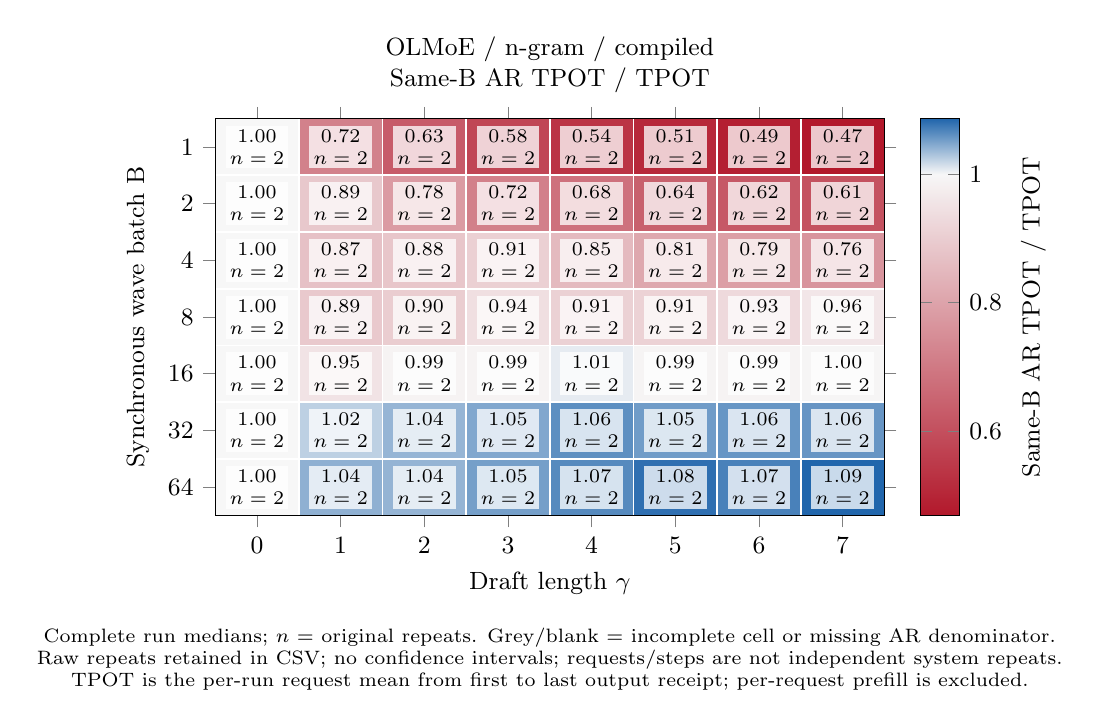
\begin{tikzpicture}
\begin{axis}[name=matrix,width=8.50cm,height=5.04cm,scale only axis,xmin=-.5,xmax=7.5,ymin=-.5,ymax=6.5,y dir=reverse,axis on top,tick align=outside,xtick={0,1,2,3,4,5,6,7},xticklabels={0,1,2,3,4,5,6,7},ytick={0,1,2,3,4,5,6},yticklabels={1,2,4,8,16,32,64},xlabel={Draft length $\gamma$},ylabel={Synchronous wave batch B},title={OLMoE / n-gram / compiled\\Same-B AR TPOT / TPOT},title style={align=center,font=\small},tick label style={font=\small},label style={font=\small},point meta min=0.468768080221,point meta max=1.08641318131,colormap={matrixcolors}{rgb255=(178,24,43); rgb255=(179,27,45); rgb255=(180,29,48); rgb255=(180,32,50); rgb255=(181,34,52); rgb255=(182,37,55); rgb255=(183,40,57); rgb255=(184,42,60); rgb255=(184,45,62); rgb255=(185,47,64); rgb255=(186,50,67); rgb255=(187,53,69); rgb255=(188,55,71); rgb255=(188,58,74); rgb255=(189,60,76); rgb255=(190,63,79); rgb255=(191,65,81); rgb255=(192,68,83); rgb255=(192,71,86); rgb255=(193,73,88); rgb255=(194,76,90); rgb255=(195,78,93); rgb255=(196,81,95); rgb255=(196,84,98); rgb255=(197,86,100); rgb255=(198,89,102); rgb255=(199,91,105); rgb255=(200,94,107); rgb255=(200,97,109); rgb255=(201,99,112); rgb255=(202,102,114); rgb255=(203,104,117); rgb255=(204,107,119); rgb255=(204,110,121); rgb255=(205,112,124); rgb255=(206,115,126); rgb255=(207,117,128); rgb255=(208,120,131); rgb255=(208,123,133); rgb255=(209,125,136); rgb255=(210,128,138); rgb255=(211,130,140); rgb255=(212,133,143); rgb255=(212,135,145); rgb255=(213,138,147); rgb255=(214,141,150); rgb255=(215,143,152); rgb255=(216,146,154); rgb255=(217,148,157); rgb255=(217,151,159); rgb255=(218,154,162); rgb255=(219,156,164); rgb255=(220,159,166); rgb255=(221,161,169); rgb255=(221,164,171); rgb255=(222,167,173); rgb255=(223,169,176); rgb255=(224,172,178); rgb255=(225,174,181); rgb255=(225,177,183); rgb255=(226,180,185); rgb255=(227,182,188); rgb255=(228,185,190); rgb255=(229,187,192); rgb255=(229,190,195); rgb255=(230,193,197); rgb255=(231,195,200); rgb255=(232,198,202); rgb255=(233,200,204); rgb255=(233,203,207); rgb255=(234,205,209); rgb255=(235,208,211); rgb255=(236,211,214); rgb255=(237,213,216); rgb255=(237,216,219); rgb255=(238,218,221); rgb255=(239,221,223); rgb255=(240,224,226); rgb255=(241,226,228); rgb255=(241,229,230); rgb255=(242,231,233); rgb255=(243,234,235); rgb255=(244,237,237); rgb255=(245,239,240); rgb255=(245,242,242); rgb255=(246,244,245); rgb255=(247,247,247); rgb255=(232,237,242); rgb255=(217,226,236); rgb255=(201,216,231); rgb255=(186,206,226); rgb255=(171,195,220); rgb255=(155,185,215); rgb255=(140,175,210); rgb255=(125,164,204); rgb255=(109,154,199); rgb255=(94,143,193); rgb255=(79,133,188); rgb255=(64,123,183); rgb255=(48,112,177); rgb255=(33,102,172)},colorbar,colorbar style={ylabel={Same-B AR TPOT / TPOT},label style={font=\small},tick label style={font=\small}}]
\path[fill={rgb,255:red,247;green,247;blue,247},draw=white,line width=.6pt] (axis cs:-0.5,-0.5) rectangle (axis cs:0.5,0.5);
\node[align=center,font=\scriptsize,fill=white,fill opacity=.76,text opacity=1,inner sep=1.5pt] at (axis cs:0,0) {1.00\\$n=2$};
\path[fill={rgb,255:red,210;green,129;blue,139},draw=white,line width=.6pt] (axis cs:0.5,-0.5) rectangle (axis cs:1.5,0.5);
\node[align=center,font=\scriptsize,fill=white,fill opacity=.76,text opacity=1,inner sep=1.5pt] at (axis cs:1,0) {0.72\\$n=2$};
\path[fill={rgb,255:red,199;green,91;blue,105},draw=white,line width=.6pt] (axis cs:1.5,-0.5) rectangle (axis cs:2.5,0.5);
\node[align=center,font=\scriptsize,fill=white,fill opacity=.76,text opacity=1,inner sep=1.5pt] at (axis cs:2,0) {0.63\\$n=2$};
\path[fill={rgb,255:red,192;green,70;blue,85},draw=white,line width=.6pt] (axis cs:2.5,-0.5) rectangle (axis cs:3.5,0.5);
\node[align=center,font=\scriptsize,fill=white,fill opacity=.76,text opacity=1,inner sep=1.5pt] at (axis cs:3,0) {0.58\\$n=2$};
\path[fill={rgb,255:red,187;green,52;blue,69},draw=white,line width=.6pt] (axis cs:3.5,-0.5) rectangle (axis cs:4.5,0.5);
\node[align=center,font=\scriptsize,fill=white,fill opacity=.76,text opacity=1,inner sep=1.5pt] at (axis cs:4,0) {0.54\\$n=2$};
\path[fill={rgb,255:red,183;green,40;blue,58},draw=white,line width=.6pt] (axis cs:4.5,-0.5) rectangle (axis cs:5.5,0.5);
\node[align=center,font=\scriptsize,fill=white,fill opacity=.76,text opacity=1,inner sep=1.5pt] at (axis cs:5,0) {0.51\\$n=2$};
\path[fill={rgb,255:red,180;green,31;blue,50},draw=white,line width=.6pt] (axis cs:5.5,-0.5) rectangle (axis cs:6.5,0.5);
\node[align=center,font=\scriptsize,fill=white,fill opacity=.76,text opacity=1,inner sep=1.5pt] at (axis cs:6,0) {0.49\\$n=2$};
\path[fill={rgb,255:red,178;green,24;blue,43},draw=white,line width=.6pt] (axis cs:6.5,-0.5) rectangle (axis cs:7.5,0.5);
\node[align=center,font=\scriptsize,fill=white,fill opacity=.76,text opacity=1,inner sep=1.5pt] at (axis cs:7,0) {0.47\\$n=2$};
\path[fill={rgb,255:red,247;green,247;blue,247},draw=white,line width=.6pt] (axis cs:-0.5,0.5) rectangle (axis cs:0.5,1.5);
\node[align=center,font=\scriptsize,fill=white,fill opacity=.76,text opacity=1,inner sep=1.5pt] at (axis cs:0,1) {1.00\\$n=2$};
\path[fill={rgb,255:red,232;green,200;blue,204},draw=white,line width=.6pt] (axis cs:0.5,0.5) rectangle (axis cs:1.5,1.5);
\node[align=center,font=\scriptsize,fill=white,fill opacity=.76,text opacity=1,inner sep=1.5pt] at (axis cs:1,1) {0.89\\$n=2$};
\path[fill={rgb,255:red,219;green,155;blue,163},draw=white,line width=.6pt] (axis cs:1.5,0.5) rectangle (axis cs:2.5,1.5);
\node[align=center,font=\scriptsize,fill=white,fill opacity=.76,text opacity=1,inner sep=1.5pt] at (axis cs:2,1) {0.78\\$n=2$};
\path[fill={rgb,255:red,210;green,128;blue,138},draw=white,line width=.6pt] (axis cs:2.5,0.5) rectangle (axis cs:3.5,1.5);
\node[align=center,font=\scriptsize,fill=white,fill opacity=.76,text opacity=1,inner sep=1.5pt] at (axis cs:3,1) {0.72\\$n=2$};
\path[fill={rgb,255:red,206;green,113;blue,125},draw=white,line width=.6pt] (axis cs:3.5,0.5) rectangle (axis cs:4.5,1.5);
\node[align=center,font=\scriptsize,fill=white,fill opacity=.76,text opacity=1,inner sep=1.5pt] at (axis cs:4,1) {0.68\\$n=2$};
\path[fill={rgb,255:red,200;green,97;blue,109},draw=white,line width=.6pt] (axis cs:4.5,0.5) rectangle (axis cs:5.5,1.5);
\node[align=center,font=\scriptsize,fill=white,fill opacity=.76,text opacity=1,inner sep=1.5pt] at (axis cs:5,1) {0.64\\$n=2$};
\path[fill={rgb,255:red,198;green,88;blue,102},draw=white,line width=.6pt] (axis cs:5.5,0.5) rectangle (axis cs:6.5,1.5);
\node[align=center,font=\scriptsize,fill=white,fill opacity=.76,text opacity=1,inner sep=1.5pt] at (axis cs:6,1) {0.62\\$n=2$};
\path[fill={rgb,255:red,196;green,82;blue,96},draw=white,line width=.6pt] (axis cs:6.5,0.5) rectangle (axis cs:7.5,1.5);
\node[align=center,font=\scriptsize,fill=white,fill opacity=.76,text opacity=1,inner sep=1.5pt] at (axis cs:7,1) {0.61\\$n=2$};
\path[fill={rgb,255:red,247;green,247;blue,247},draw=white,line width=.6pt] (axis cs:-0.5,1.5) rectangle (axis cs:0.5,2.5);
\node[align=center,font=\scriptsize,fill=white,fill opacity=.76,text opacity=1,inner sep=1.5pt] at (axis cs:0,2) {1.00\\$n=2$};
\path[fill={rgb,255:red,230;green,193;blue,198},draw=white,line width=.6pt] (axis cs:0.5,1.5) rectangle (axis cs:1.5,2.5);
\node[align=center,font=\scriptsize,fill=white,fill opacity=.76,text opacity=1,inner sep=1.5pt] at (axis cs:1,2) {0.87\\$n=2$};
\path[fill={rgb,255:red,232;green,198;blue,202},draw=white,line width=.6pt] (axis cs:1.5,1.5) rectangle (axis cs:2.5,2.5);
\node[align=center,font=\scriptsize,fill=white,fill opacity=.76,text opacity=1,inner sep=1.5pt] at (axis cs:2,2) {0.88\\$n=2$};
\path[fill={rgb,255:red,235;green,208;blue,211},draw=white,line width=.6pt] (axis cs:2.5,1.5) rectangle (axis cs:3.5,2.5);
\node[align=center,font=\scriptsize,fill=white,fill opacity=.76,text opacity=1,inner sep=1.5pt] at (axis cs:3,2) {0.91\\$n=2$};
\path[fill={rgb,255:red,228;green,186;blue,191},draw=white,line width=.6pt] (axis cs:3.5,1.5) rectangle (axis cs:4.5,2.5);
\node[align=center,font=\scriptsize,fill=white,fill opacity=.76,text opacity=1,inner sep=1.5pt] at (axis cs:4,2) {0.85\\$n=2$};
\path[fill={rgb,255:red,222;green,168;blue,174},draw=white,line width=.6pt] (axis cs:4.5,1.5) rectangle (axis cs:5.5,2.5);
\node[align=center,font=\scriptsize,fill=white,fill opacity=.76,text opacity=1,inner sep=1.5pt] at (axis cs:5,2) {0.81\\$n=2$};
\path[fill={rgb,255:red,220;green,159;blue,166},draw=white,line width=.6pt] (axis cs:5.5,1.5) rectangle (axis cs:6.5,2.5);
\node[align=center,font=\scriptsize,fill=white,fill opacity=.76,text opacity=1,inner sep=1.5pt] at (axis cs:6,2) {0.79\\$n=2$};
\path[fill={rgb,255:red,216;green,148;blue,157},draw=white,line width=.6pt] (axis cs:6.5,1.5) rectangle (axis cs:7.5,2.5);
\node[align=center,font=\scriptsize,fill=white,fill opacity=.76,text opacity=1,inner sep=1.5pt] at (axis cs:7,2) {0.76\\$n=2$};
\path[fill={rgb,255:red,247;green,247;blue,247},draw=white,line width=.6pt] (axis cs:-0.5,2.5) rectangle (axis cs:0.5,3.5);
\node[align=center,font=\scriptsize,fill=white,fill opacity=.76,text opacity=1,inner sep=1.5pt] at (axis cs:0,3) {1.00\\$n=2$};
\path[fill={rgb,255:red,233;green,201;blue,205},draw=white,line width=.6pt] (axis cs:0.5,2.5) rectangle (axis cs:1.5,3.5);
\node[align=center,font=\scriptsize,fill=white,fill opacity=.76,text opacity=1,inner sep=1.5pt] at (axis cs:1,3) {0.89\\$n=2$};
\path[fill={rgb,255:red,234;green,205;blue,208},draw=white,line width=.6pt] (axis cs:1.5,2.5) rectangle (axis cs:2.5,3.5);
\node[align=center,font=\scriptsize,fill=white,fill opacity=.76,text opacity=1,inner sep=1.5pt] at (axis cs:2,3) {0.90\\$n=2$};
\path[fill={rgb,255:red,240;green,223;blue,225},draw=white,line width=.6pt] (axis cs:2.5,2.5) rectangle (axis cs:3.5,3.5);
\node[align=center,font=\scriptsize,fill=white,fill opacity=.76,text opacity=1,inner sep=1.5pt] at (axis cs:3,3) {0.94\\$n=2$};
\path[fill={rgb,255:red,235;green,209;blue,212},draw=white,line width=.6pt] (axis cs:3.5,2.5) rectangle (axis cs:4.5,3.5);
\node[align=center,font=\scriptsize,fill=white,fill opacity=.76,text opacity=1,inner sep=1.5pt] at (axis cs:4,3) {0.91\\$n=2$};
\path[fill={rgb,255:red,236;green,210;blue,213},draw=white,line width=.6pt] (axis cs:4.5,2.5) rectangle (axis cs:5.5,3.5);
\node[align=center,font=\scriptsize,fill=white,fill opacity=.76,text opacity=1,inner sep=1.5pt] at (axis cs:5,3) {0.91\\$n=2$};
\path[fill={rgb,255:red,238;green,217;blue,220},draw=white,line width=.6pt] (axis cs:5.5,2.5) rectangle (axis cs:6.5,3.5);
\node[align=center,font=\scriptsize,fill=white,fill opacity=.76,text opacity=1,inner sep=1.5pt] at (axis cs:6,3) {0.93\\$n=2$};
\path[fill={rgb,255:red,242;green,230;blue,232},draw=white,line width=.6pt] (axis cs:6.5,2.5) rectangle (axis cs:7.5,3.5);
\node[align=center,font=\scriptsize,fill=white,fill opacity=.76,text opacity=1,inner sep=1.5pt] at (axis cs:7,3) {0.96\\$n=2$};
\path[fill={rgb,255:red,247;green,247;blue,247},draw=white,line width=.6pt] (axis cs:-0.5,3.5) rectangle (axis cs:0.5,4.5);
\node[align=center,font=\scriptsize,fill=white,fill opacity=.76,text opacity=1,inner sep=1.5pt] at (axis cs:0,4) {1.00\\$n=2$};
\path[fill={rgb,255:red,241;green,227;blue,229},draw=white,line width=.6pt] (axis cs:0.5,3.5) rectangle (axis cs:1.5,4.5);
\node[align=center,font=\scriptsize,fill=white,fill opacity=.76,text opacity=1,inner sep=1.5pt] at (axis cs:1,4) {0.95\\$n=2$};
\path[fill={rgb,255:red,246;green,243;blue,243},draw=white,line width=.6pt] (axis cs:1.5,3.5) rectangle (axis cs:2.5,4.5);
\node[align=center,font=\scriptsize,fill=white,fill opacity=.76,text opacity=1,inner sep=1.5pt] at (axis cs:2,4) {0.99\\$n=2$};
\path[fill={rgb,255:red,246;green,243;blue,243},draw=white,line width=.6pt] (axis cs:2.5,3.5) rectangle (axis cs:3.5,4.5);
\node[align=center,font=\scriptsize,fill=white,fill opacity=.76,text opacity=1,inner sep=1.5pt] at (axis cs:3,4) {0.99\\$n=2$};
\path[fill={rgb,255:red,230;green,235;blue,241},draw=white,line width=.6pt] (axis cs:3.5,3.5) rectangle (axis cs:4.5,4.5);
\node[align=center,font=\scriptsize,fill=white,fill opacity=.76,text opacity=1,inner sep=1.5pt] at (axis cs:4,4) {1.01\\$n=2$};
\path[fill={rgb,255:red,246;green,244;blue,244},draw=white,line width=.6pt] (axis cs:4.5,3.5) rectangle (axis cs:5.5,4.5);
\node[align=center,font=\scriptsize,fill=white,fill opacity=.76,text opacity=1,inner sep=1.5pt] at (axis cs:5,4) {0.99\\$n=2$};
\path[fill={rgb,255:red,246;green,243;blue,243},draw=white,line width=.6pt] (axis cs:5.5,3.5) rectangle (axis cs:6.5,4.5);
\node[align=center,font=\scriptsize,fill=white,fill opacity=.76,text opacity=1,inner sep=1.5pt] at (axis cs:6,4) {0.99\\$n=2$};
\path[fill={rgb,255:red,246;green,245;blue,245},draw=white,line width=.6pt] (axis cs:6.5,3.5) rectangle (axis cs:7.5,4.5);
\node[align=center,font=\scriptsize,fill=white,fill opacity=.76,text opacity=1,inner sep=1.5pt] at (axis cs:7,4) {1.00\\$n=2$};
\path[fill={rgb,255:red,247;green,247;blue,247},draw=white,line width=.6pt] (axis cs:-0.5,4.5) rectangle (axis cs:0.5,5.5);
\node[align=center,font=\scriptsize,fill=white,fill opacity=.76,text opacity=1,inner sep=1.5pt] at (axis cs:0,5) {1.00\\$n=2$};
\path[fill={rgb,255:red,189;green,208;blue,227},draw=white,line width=.6pt] (axis cs:0.5,4.5) rectangle (axis cs:1.5,5.5);
\node[align=center,font=\scriptsize,fill=white,fill opacity=.76,text opacity=1,inner sep=1.5pt] at (axis cs:1,5) {1.02\\$n=2$};
\path[fill={rgb,255:red,150;green,181;blue,213},draw=white,line width=.6pt] (axis cs:1.5,4.5) rectangle (axis cs:2.5,5.5);
\node[align=center,font=\scriptsize,fill=white,fill opacity=.76,text opacity=1,inner sep=1.5pt] at (axis cs:2,5) {1.04\\$n=2$};
\path[fill={rgb,255:red,129;green,167;blue,206},draw=white,line width=.6pt] (axis cs:2.5,4.5) rectangle (axis cs:3.5,5.5);
\node[align=center,font=\scriptsize,fill=white,fill opacity=.76,text opacity=1,inner sep=1.5pt] at (axis cs:3,5) {1.05\\$n=2$};
\path[fill={rgb,255:red,93;green,143;blue,193},draw=white,line width=.6pt] (axis cs:3.5,4.5) rectangle (axis cs:4.5,5.5);
\node[align=center,font=\scriptsize,fill=white,fill opacity=.76,text opacity=1,inner sep=1.5pt] at (axis cs:4,5) {1.06\\$n=2$};
\path[fill={rgb,255:red,112;green,156;blue,200},draw=white,line width=.6pt] (axis cs:4.5,4.5) rectangle (axis cs:5.5,5.5);
\node[align=center,font=\scriptsize,fill=white,fill opacity=.76,text opacity=1,inner sep=1.5pt] at (axis cs:5,5) {1.05\\$n=2$};
\path[fill={rgb,255:red,103;green,150;blue,197},draw=white,line width=.6pt] (axis cs:5.5,4.5) rectangle (axis cs:6.5,5.5);
\node[align=center,font=\scriptsize,fill=white,fill opacity=.76,text opacity=1,inner sep=1.5pt] at (axis cs:6,5) {1.06\\$n=2$};
\path[fill={rgb,255:red,103;green,149;blue,196},draw=white,line width=.6pt] (axis cs:6.5,4.5) rectangle (axis cs:7.5,5.5);
\node[align=center,font=\scriptsize,fill=white,fill opacity=.76,text opacity=1,inner sep=1.5pt] at (axis cs:7,5) {1.06\\$n=2$};
\path[fill={rgb,255:red,247;green,247;blue,247},draw=white,line width=.6pt] (axis cs:-0.5,5.5) rectangle (axis cs:0.5,6.5);
\node[align=center,font=\scriptsize,fill=white,fill opacity=.76,text opacity=1,inner sep=1.5pt] at (axis cs:0,6) {1.00\\$n=2$};
\path[fill={rgb,255:red,143;green,176;blue,210},draw=white,line width=.6pt] (axis cs:0.5,5.5) rectangle (axis cs:1.5,6.5);
\node[align=center,font=\scriptsize,fill=white,fill opacity=.76,text opacity=1,inner sep=1.5pt] at (axis cs:1,6) {1.04\\$n=2$};
\path[fill={rgb,255:red,149;green,180;blue,212},draw=white,line width=.6pt] (axis cs:1.5,5.5) rectangle (axis cs:2.5,6.5);
\node[align=center,font=\scriptsize,fill=white,fill opacity=.76,text opacity=1,inner sep=1.5pt] at (axis cs:2,6) {1.04\\$n=2$};
\path[fill={rgb,255:red,117;green,159;blue,201},draw=white,line width=.6pt] (axis cs:2.5,5.5) rectangle (axis cs:3.5,6.5);
\node[align=center,font=\scriptsize,fill=white,fill opacity=.76,text opacity=1,inner sep=1.5pt] at (axis cs:3,6) {1.05\\$n=2$};
\path[fill={rgb,255:red,86;green,138;blue,190},draw=white,line width=.6pt] (axis cs:3.5,5.5) rectangle (axis cs:4.5,6.5);
\node[align=center,font=\scriptsize,fill=white,fill opacity=.76,text opacity=1,inner sep=1.5pt] at (axis cs:4,6) {1.07\\$n=2$};
\path[fill={rgb,255:red,47;green,111;blue,177},draw=white,line width=.6pt] (axis cs:4.5,5.5) rectangle (axis cs:5.5,6.5);
\node[align=center,font=\scriptsize,fill=white,fill opacity=.76,text opacity=1,inner sep=1.5pt] at (axis cs:5,6) {1.08\\$n=2$};
\path[fill={rgb,255:red,73;green,129;blue,186},draw=white,line width=.6pt] (axis cs:5.5,5.5) rectangle (axis cs:6.5,6.5);
\node[align=center,font=\scriptsize,fill=white,fill opacity=.76,text opacity=1,inner sep=1.5pt] at (axis cs:6,6) {1.07\\$n=2$};
\path[fill={rgb,255:red,33;green,102;blue,172},draw=white,line width=.6pt] (axis cs:6.5,5.5) rectangle (axis cs:7.5,6.5);
\node[align=center,font=\scriptsize,fill=white,fill opacity=.76,text opacity=1,inner sep=1.5pt] at (axis cs:7,6) {1.09\\$n=2$};
\end{axis}
\node[below=1.3cm,align=center,font=\scriptsize] at (matrix.south) {Complete run medians; $n$ = original repeats. Grey/blank = incomplete cell or missing AR denominator.\\Raw repeats retained in CSV; no confidence intervals; requests/steps are not independent system repeats.\\TPOT is the per-run request mean from first to last output receipt; per-request prefill is excluded.};
\end{tikzpicture}\end{document}
